
The overall idea of the proposed decomposition methodology is to break down the system and/or the verification into sub-parts that can be solved independently regarding the properties to be validated over the whole system.

The hard part of the model checking decomposition is to find how to decompose while preserving a consistent expression of "local" properties with regards to the "global" ones. While the decomposition criteria provided here are specific to the Precision Spraying Problem, the intent is to propose a generic decomposition method that can be used for decision support in other agricultural domains or beyond.

The decomposition of a model checking problem should consist in three phases: the decomposition of the model (modelling decomposition), the decomposition of the verification process (verification decomposition) and the analysis of the decomposition (decomposition analysis). Modelling decomposition partitions the model into n sub-models. 2 sub-models may have an overlap zone in common and this will be detailed in section \ref{MD}.

The decomposition of verification is about decomposing the resolution of the property to be checked on the global model into the resolution of properties on the sub-models. The decomposition analysis is about proving that this verification of the properties on the sub-models guaranties the verification of the initial property on the global model.

The outline of the section follows the 3 above-mentioned phases.

\subsection{Modelling Decomposition}
\label{MD}

The modelling decomposition consists in decomposing the model into $n$ parts. One or several criteria for decomposition need to be found out in order to proceed to this.

\paragraph{\textbf{Decomposition criterion}} 

The intrinsic spatial characteristics of the agricultural applications provide guidance for decomposing. The geometrical structure of most of the agricultural fields is a useful element for decomposition. In the Precision Spraying problem, considering that each row is sprayed independently, step 3 of AMPS methodology can be applied separately to each row. The decomposition of a model including $n$ rows to $n$ models including each a unique row is thus straightforward. On the practical side, the model presented in \ref{Verif} was designed for one row, with a set of data for each row of the studied field.
Steps 1 and 2 of AMPS are better applied at a larger scale (field or vineyard) in order to have consistent crop protection of the vineyard.

Other characteristics may be used to find a decomposition criterion, depending on the application cases. The idea is to find an agricultural characteristic that imposes a fixed and known value in the verification process. This value will be the pivot of the decomposition strategy for verification.
In the Precision Spraying case, where an optimal spraying command sequence is searched, the optimal command sequence before the pivot should be independent of the optimal command sequence after it. From this idea, two criteria were identified for the Precision Spraying problem in order to decompose the verification of a row.
The first one relates to blocks with missing vegetation. The command to be applied in this case is to close all the nozzles. This criterion is close to the spatial decomposition of the different rows, as the nozzles are closed between two rows, with the significant difference that sub-systems overlap on missing vegetation blocks. The impact of overlapping will be explained hereafter.

A criterion that is more complex to handle can be extracted considering the PSM function. The presence of a block where $C_{best}$ = $C_{alt}$ in a row represents a case where the command to apply is known a priori. These blocks allow to break the dependency between the sequence of commands before and after them, which is the basic need for the decomposition process. The MC decomposition based on the criterion $C_{best}$ $=$ $C_{alt}$ is the most complex with regards to the three phases of decomposition and is detailed in the following.

\paragraph{\textbf{Forming row parts}} 
A row part is a subset of successive blocks of a row. The row parts are defined so that there is an overlapping block that belongs to two successive parts. The case considered here is the case where an overlapping block has the property that $C_{best}$ = $C_{alt}$). Such block will be called hereafter a "same command block".

Thus, a row $R$ is decomposed into $ n $ parts $ \{P_1$, ..., $P_n\}$. Each $P_i$ is a set of blocks which begins with a block where $C_{best}$ = $C_{alt}$ or with the first block of the row, and which ends with a block where $C_{best}$ = $C_{alt}$ or with the last block of the row.

The figure \ref{fig:decompo_in_two} illustrates, by an example, the formation of the row parts.

The hypothetical example row $R$ is formed of $5$ blocks. The block $\{b_{3}$ is a same command block ($C_{best}$ = $C_{alt}$). The part $P_{A}$ is made up of blocks $b_{1}$,$b_{2}$ and $b_{3}$. The part $ P_{B} $ starts from block $b_{3}$ included and contains also $b_{4}$ and $b_{5}$. $b_{3}$ is the overlapping block.

\begin{figure}[h!]
	\begin{center}
		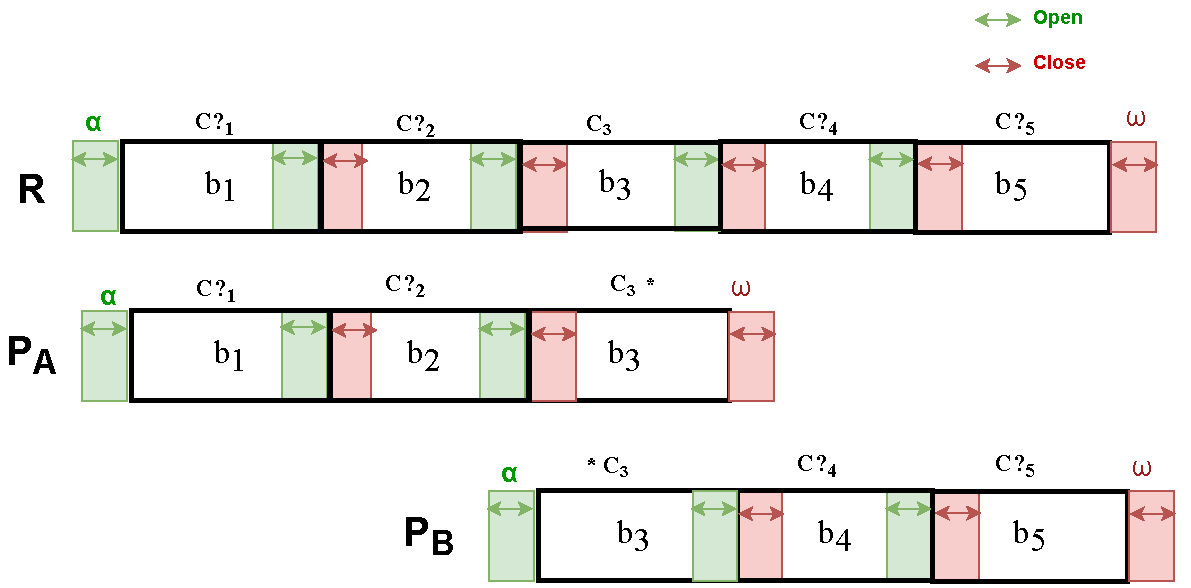
\includegraphics[width=7.2cm]{decompo2.pdf} 
		\caption{Decomposition of row $R$ in two parts} 
		\label{fig:decompo_in_two}
	\end{center}
\end{figure} 

\textbf{Generating sub-models}. Using the $PTA\_PSP$ model for UPPAAL-CORA, the generation of the sub-models for each row part consists only in editing the input data of the model. No change is needed in the description of the automata. The global constants describing commands are updated with information related to the corresponding row part: the value of the number of blocks forming the row is replaced with the value of the number of blocks forming the part (constant \texttt{nb$\_$block}); and all the tables storing the information of these blocks will be updated with only the concerned blocks.
It is worth noting that, as the configuration of the models is based on text files, the modelling decomposition is automated. It is also important to have in mind that, because the model of a part of a row is a model of a row with a reduced number of blocks, some parts have a "virtual row ending" (part $P_A$ in figure \ref{fig:decompo_in_two}) and some have a "virtual row beginning" (parts $P_B$ in same figure). Real beginnings and endings of rows have the characteristic that all the nozzles should be off before and after spraying the row. Technically, in the model of a part of a row, this constraint is also applied to its virtual beginning and its virtual ending. The consequences of this for calculating the optimal sequence and the optimal cost for a whole row from the optimal sequences and optimal costs for the parts are analysed in section \ref{PreveComp}.


\subsection{Verification Decomposition}
\label{VD}
The verification decomposition decomposes the resolution of the property to be checked on the global model into the resolution of properties on the sub-models.

Let us recall that the property allowing to obtain the optimal command sequence applied on all the rows is the property \texttt{PP1} 
described in the section \ref{sec:VerifProp}. The verification process on the sub-models is based on the same property, but with the modifications of the models previously mentioned.

The decomposition of the verification consists in verifying this property on each row part. It is important to note that in the model of a part, $ nb\_block $ becomes the number of blocks forming the part and $ StartRowAut.end $ is reached when the sprayer finishes spraying all the blocks of the part. 

Checking the property \texttt{PP1} on the sub-model allows to calculate the Optimal Sequence to be applied on the part and to calculate its Optimal Cost. 
The complete optimal sequence can be calculated from the concatenation of the optimal sequences of the parts, and the global optimal cost can be calculated from the sum of the optimal costs of the parts. Rules for concatenation and cost rectification terms respectively required in these operations when overlapping occurs in decomposition (see figure \ref{fig:decompo_in_two}) will be explicited hereafter.

\subsection{Decomposition Analysis}
\label{PreveComp}

The decomposition analysis is about proving that the verification of the properties on the sub-models allows the verification of the initial property on the global model.
Let us consider a row, or row part such as in figure \ref{fig:decompo_in_two}, which can described by equation \ref{eq:SRExample_r}:

\begin{equation}
	S_R = \oslash \triangleright C?_{1} \triangleright C?_{2} \triangleright C_{3} \triangleright C?_{4} \triangleright C?_{5} \triangleright \oslash \label{eq:SRExample_r}
\end{equation}

In equation \ref{eq:SRExample_r}, $\oslash$ means that all nozzles are off. $C?_{i}$ denotes a choice to make for block $b_i$ and $C_{i}$ is the command for block $b_{i}$ when it has a unique possibility. The decomposition can be made here using block $b_3$ as overlapping block.  Sequences $S_A$ and $S_B$ for the resulting parts $P_A$ and $P_B$ can be written:
\begin{eqnarray}
	&S_A =& \oslash \triangleright C?_1 \triangleright C?_2 \triangleright C_{3}* \triangleright \oslash \label{eq:SAExample_r}
	\\
	&S_B =& \oslash \triangleright *C_{3} \triangleright C?_4 \triangleright C?_5 \triangleright \oslash \label{eq:SBExample_r}
\end{eqnarray}

The symbol $*$ either on the left or on the right of $C_3$ denotes that overlapping occurs here. The concatenation law for parts having an overlapping is given in equation \ref{eq:ruleconcatparts}. It can easily be shown that when applying this concatenation law to $S_A$ and $S_B$, then $S_R = S_A \triangleright S_B$.

\begin{equation}
	C* \triangleright \oslash \triangleright \oslash \triangleright *C = C \label{eq:ruleconcatparts}
\end{equation}

Now, as written in equation \ref{eq:costcorrection}, the rectification terms for calculating the cost of $S_R$ from the costs obtained for $S_A$ and $S_B$ once solved by CORA algorithm can be formulated. Considering that the cost for $C_3$ has been counted once in $S_A$ with $C_3 *$ and once again in $S_B$ with $*C_3$ then the cost $Q_{3}(C_{3})$ of this command should be retrieved from the sum of costs of parts. Considering also that there was no actual closing and re-opening of nozzles for $C_3$ between $C_3 *$ and $*C_3$, the formulation of the cost correction term is provided in equation \ref{eq:correctionterm}. This reasoning applies to any decomposition of a row in $n$ parts by simple recursion of cutting a part in two. The calculation of optimal cost of a row from optimal sequences on $n$ row parts is thus demonstrated.

\begin{equation}
	c(S_A \triangleright S_B)=c(S_A)+c(S_B)+corr(S_A \triangleright S_B) \label{eq:costcorrection}
\end{equation}
%\vspace{-1em}
\begin{equation}
	corr(S_A \triangleright S_B)= - Q_{3}(C_{3}) - close(C_{3}) - open(C_{3}) \label{eq:correctionterm}
\end{equation}

In this section, it was shown how to proceed to model-checking decomposition.
In section \ref{results}, the decomposition methodology will be applied on a real vine plot. The next section details the data acquisition system and presents the vineyard on which our precision spraying approach will be tested.


